\section{Các công trình nghiên cứu có liên quan}\label{sec:related_works}
\frame{\tableofcontents[currentsection]}

\subsection{Mạng GANs}
\begin{frame}{Mạng GANs}
\begin{figure}[H]
    \centering
    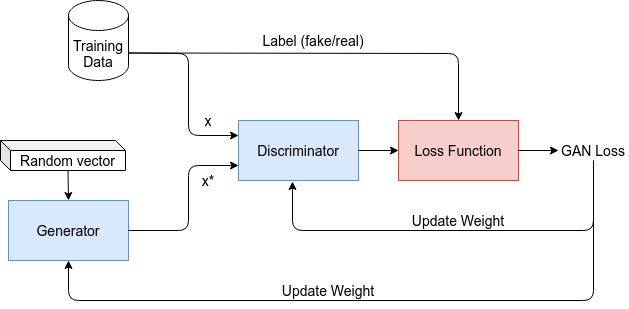
\includegraphics[width=12cm]{./images/gans-pure.png}
    \caption{Cấu trúc mạng GANs cơ bản}
    \label{fig:pure-gans}
\end{figure}
\end{frame}

\begin{frame}{Mạng GANs}
\begin{figure}[H]
    \centering
    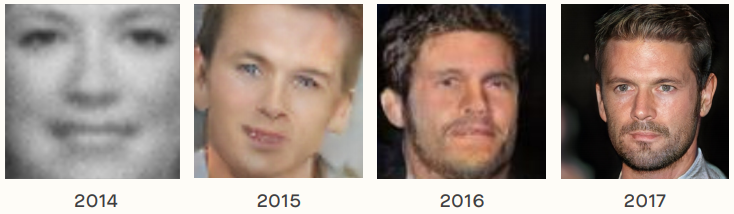
\includegraphics[width=14cm]{./images/gans-faces.png}
    \caption{Tạo sinh hình ảnh mặt người bằng mạng GANs theo các năm}
    \label{fig:gans-faces}
\end{figure}
\end{frame}

\subsection{Tổng quan tình hình nghiên cứu}
\begin{frame}{Tổng quan tình hình nghiên cứu}
\begin{figure}[H]
    \centering
    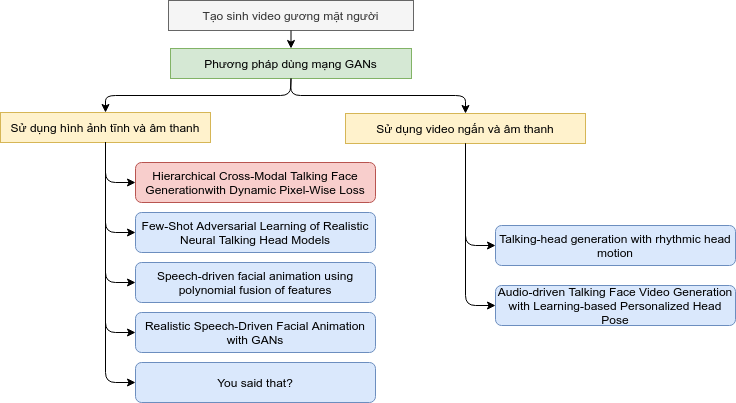
\includegraphics[width=12.5cm]{images/related_work_tree.png}
    \caption{Tổng quan tình hình nghiên cứu}
    \label{fig:related_work_tree}
\end{figure}
\end{frame}

\subsection{Nghiên cứu Hierarchical Cross-Modal Talking Face Generation With Dynamic Pixel-Wise Loss \cite{chen2019}}

\begin{frame}{Nghiên cứu Hierarchical Cross-Modal Talking Face Generation With Dynamic Pixel-Wise Loss \cite{chen2019}}
    \begin{figure}[H]
    \centering
    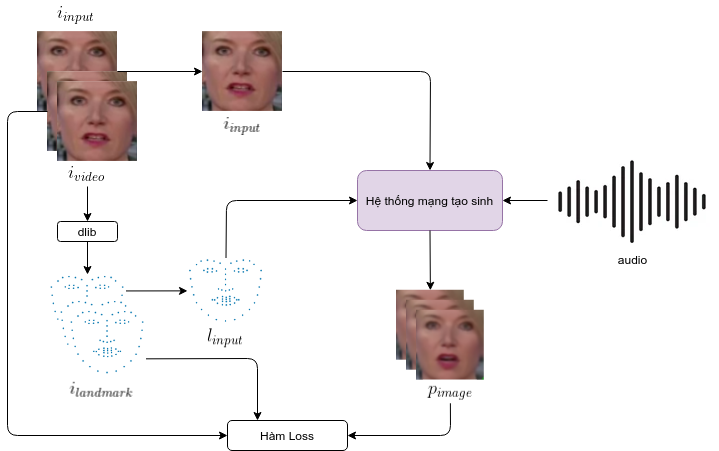
\includegraphics[width=10cm]{images/processing-training.png}
    \label{fig:processing-training}
    \caption{Phương thức tạo sinh hình ảnh}
    \end{figure}
\end{frame}

\begin{frame}{Nghiên cứu Hierarchical Cross-Modal Talking Face Generation With Dynamic Pixel-Wise Loss \cite{chen2019}}
    \begin{figure}[H]
    \centering
    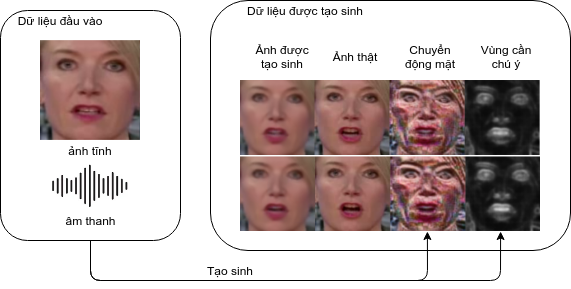
\includegraphics[width=12cm]{images/idea-small.png}
    \label{fig:idea}
    \caption{Ý tưởng tạo sinh hình ảnh từ ảnh gốc}
    \end{figure}
\end{frame}

\begin{frame}{Nghiên cứu Hierarchical Cross-Modal Talking Face Generation With Dynamic Pixel-Wise Loss \cite{chen2019}}
Hệ thống gồm có hai thành phần chính:
\begin{itemize}
    \item Mạng dự đoán cột mốc gương mặt ($\Psi$)
    \item Hệ thống mạng GANs:
    \begin{itemize}
        \item Mạng tạo sinh video ($G$)
        \item Mạng phân biệt ($D$)
    \end{itemize}
\end{itemize}
\end{frame}

\begin{frame}{Nghiên cứu Hierarchical Cross-Modal Talking Face Generation With Dynamic Pixel-Wise Loss \cite{chen2019}}
    \begin{figure}[H]
    \centering
    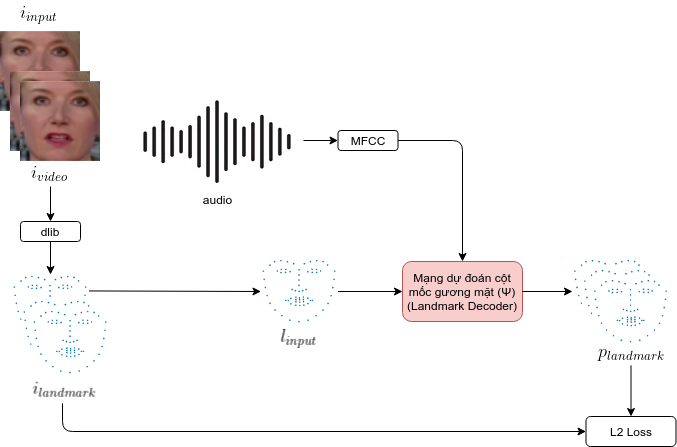
\includegraphics[width=9.5cm]{images/processing-landmark_dec.png}
    \label{fig:processing-landmark_dec}
    \caption{Mạng dự đoán cột mốc gương mặt}
    \end{figure}
\end{frame}

\begin{frame}{Nghiên cứu Hierarchical Cross-Modal Talking Face Generation With Dynamic Pixel-Wise Loss \cite{chen2019}}
    \begin{figure}[H]
    \centering
    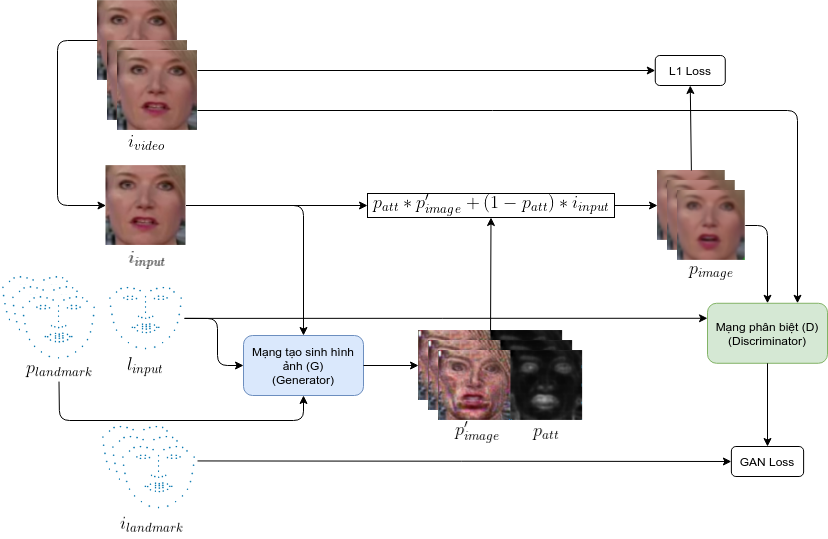
\includegraphics[width=9.5cm]{images/processing-gan.png}
    \label{fig:processing-gan}
    \caption{Mạng GANs}
    \end{figure}
\end{frame}

\begin{frame}{Cấu trúc bộ dự đoán cột mốc gương mặt (Landmark Decoder)}
    \begin{figure}[H]
        \centering
        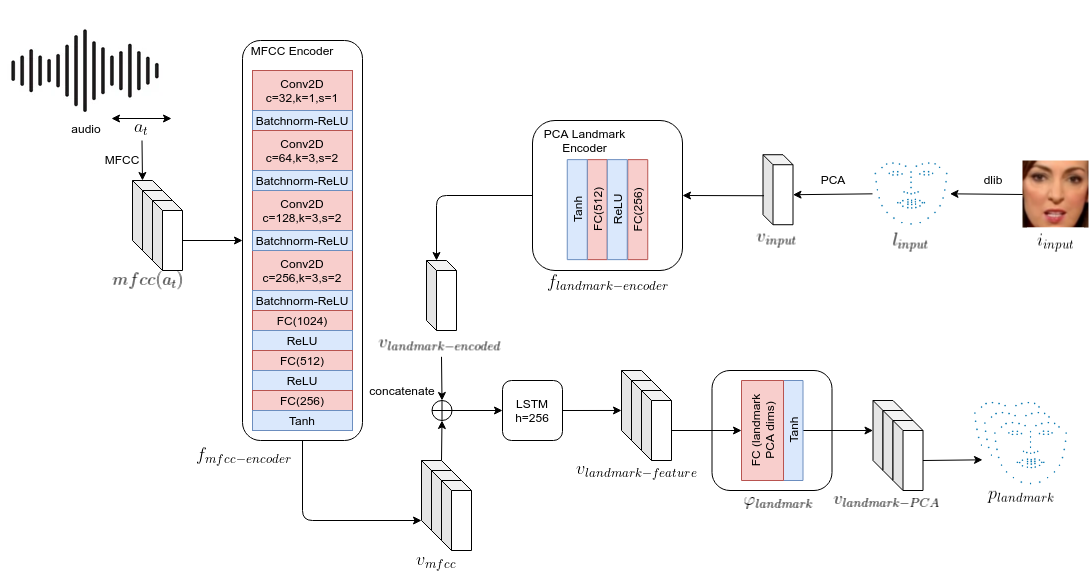
\includegraphics[width=13cm]{images/landmark_decoder.png}
        \label{fig:landmark_decoder}
        \caption{Cấu trúc bộ dự đoán cột mốc gương mặt (Landmark Decoder)}
    \end{figure}
\end{frame}

\begin{frame}{Cấu trúc bộ tạo sinh hình ảnh (Generator)}
    \begin{figure}[H]
        \centering
        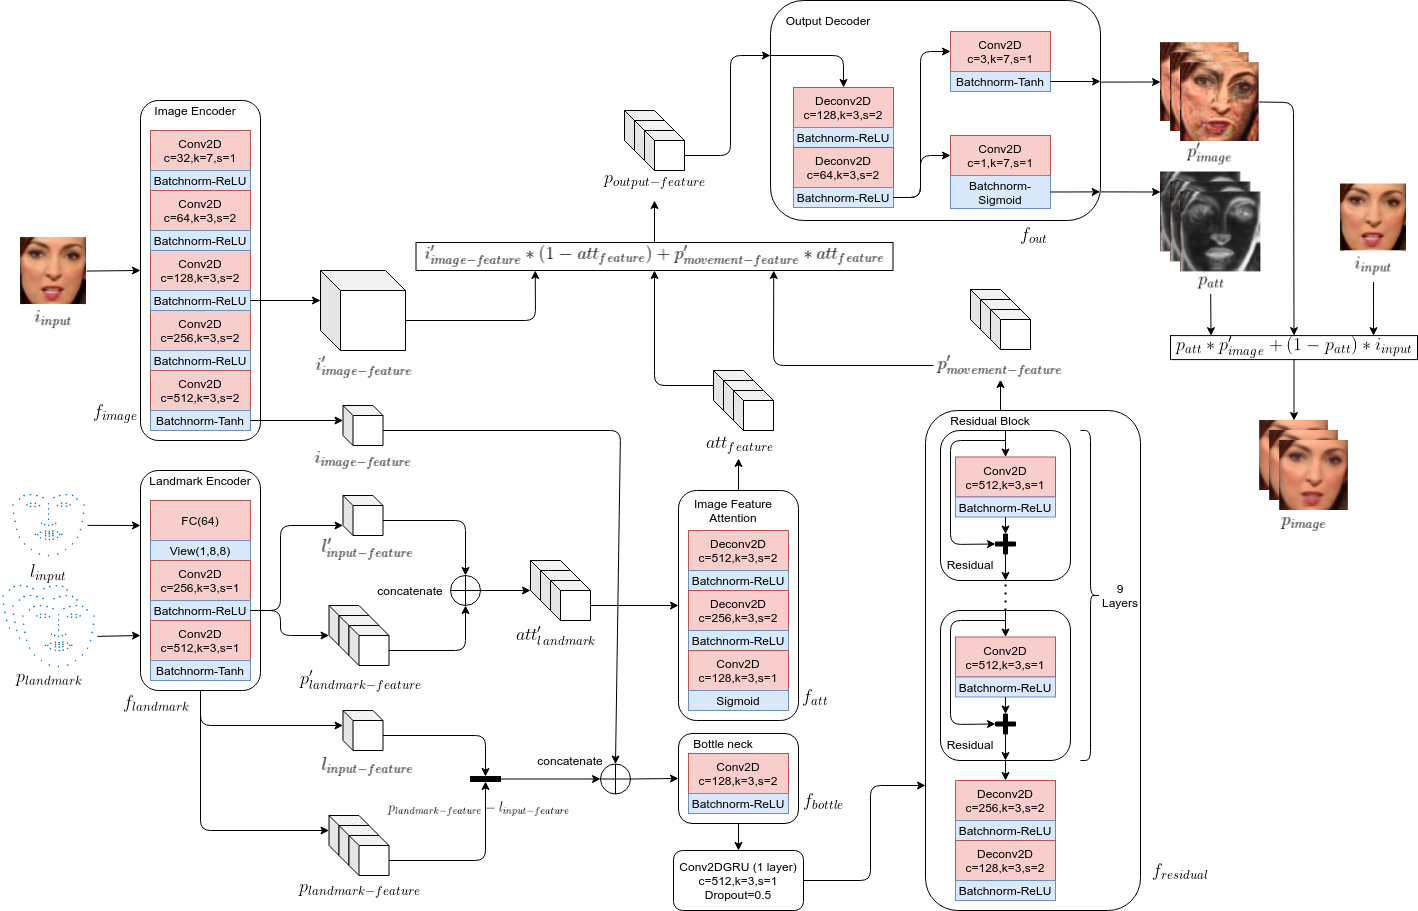
\includegraphics[width=10.5cm]{images/generator.png}
        \label{fig:generator}
        \caption{Cấu trúc bộ tạo sinh hình ảnh (Generator)}
    \end{figure}
\end{frame}

\begin{frame}{Cấu trúc bộ phân biệt (Discriminator)}
    \begin{figure}[H]
        \centering
        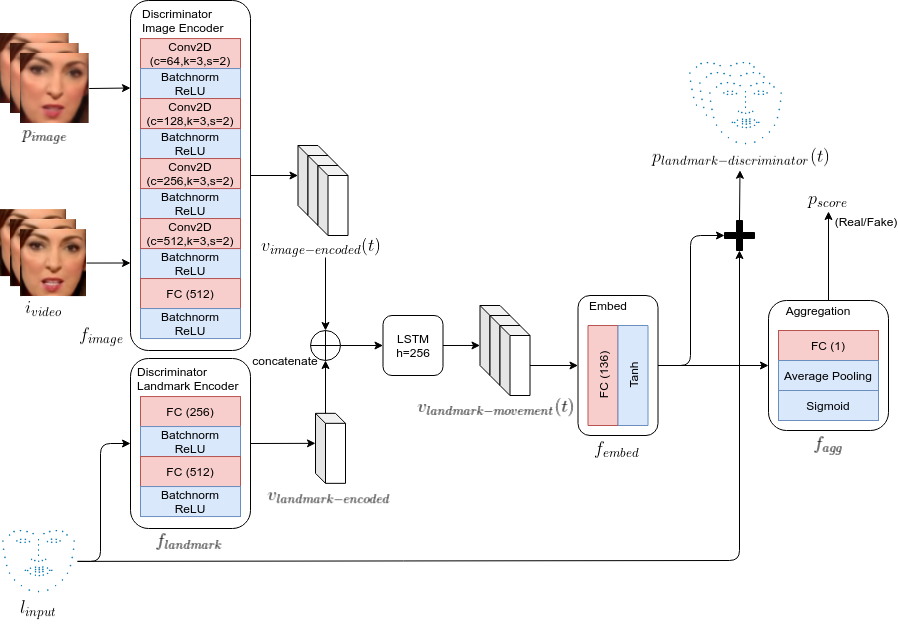
\includegraphics[width=10cm]{images/discriminator.png}
        \label{fig:discriminator}
        \caption{Cấu trúc bộ phân biệt (Discriminator)}
    \end{figure}
\end{frame}

\begin{frame}{Hàm mất mát tổng}
    \begin{equation}
        \begin{split}
        \mathcal{L}_{gans} = &\mathcal{L}_{gans-dis} + \mathcal{L}_{gans-landmark}\\
        \mathcal{L} = &\mathcal{L}_{gans} + \lambda*\mathcal{L}_{pix}
        \end{split}
    \end{equation}
    Bằng thực nghiệm ta chọn $\lambda = 10$ để cân bằng giữa $\mathcal{L}_{gans}$ và $\mathcal{L}_{pix}$
\end{frame}

\begin{frame}{Hàm mất mát cho từng pixel}
    \begin{equation}
        \mathcal{L}_{pix} = \frac{1}{T}\sum^T_{t=1}||(i_{video}(t)-p_{image}(t))*(p_{att}(t)+\beta)||_1
    \end{equation}
    
    Trong đó:
    \begin{itemize}
        \item \textbf{$i_{video}(t)$}: khung hình tại thời điểm $t$ của video gốc
        \item \textbf{$p_{image}(t)$}: hình ảnh được tạo sinh tại thời điểm $t$
        \item \textbf{$p_{att}(t)$}: mặt nạ chú ý được dự đoán tại thời điểm $t$
        \item \textbf{$\beta$}: một hằng số để đảm bảo tất cả các điểm trên ảnh đều được học, bằng thực nghiệm ta chọn $\beta = 0.5$ 
    \end{itemize}
    
\end{frame}

\begin{frame}{Hàm mất mát GANs cho bộ phân biệt}
    \begin{equation}
        \begin{split}
        \mathcal{L}_{gans-dis} = &\mathbb{E}_{l_{input},i_{video}}[logD_s(l_{input},i_{video})]\\
        +&\mathbb{E}_{l_{input},i_{input},p_{landmark}}[log(1-D_s(l_{input},G(l_{input},i_{input},p_{landmark})))]
        \end{split}
    \end{equation}
    Trong đó:
    \begin{itemize}
        \item \textbf{$l_{input},i_{input},p_{landmark},i_{video}$}: đã được giải thích ở các phần trên
        \item \textbf{$D_s$}: Mạng phân biệt với đầu ra là xác suất ảnh là ảnh thật
        \item \textbf{$G$}: Mạng tạo sinh hình ảnh
    \end{itemize}
\end{frame}

\begin{frame}{Hàm mất mát GANs cho bộ phân biệt}
\begin{equation}
    \begin{split}
    \mathcal{L}_{gans-landmark} = &||(D_l(l_{input},G(l_{input},i_{input},p_{landmark})) - l_{orig})*M_l||^2_2\\
    +&||(D_l(l_{input},i_{video}) - l_{orig})*M_l||^2_2\\
    \end{split}
\end{equation}

    Trong đó:
    \begin{itemize}
        \item \textbf{$l_{input},i_{input},p_{landmark},i_{video}$}: đã được giải thích ở các phần trên
        \item \textbf{$D_l$}: Mạng phân biệt với đầu ra là cột mốc gương mặt trên ảnh được tạo sinh
        \item \textbf{$G$}: Mạng tạo sinh hình ảnh
        \item \textbf{$l_{original}$}: Cột mốc gương mặt được trích xuất nguyên gốc từ video $i_{video}$
        \item \textbf{$M_l$}: mặt nạ nhằm chú ý nhiều hơn vào cột mốc gương mặt vùng miệng, theo đó, sai số của cột mốc ở vùng miệng có hệ số 100, trong khi các vùng khác là 1.
    \end{itemize}
\end{frame}

\begin{frame}{Tiền xử lý dữ liệu}
    Dữ liệu huấn luyện là các video với mặt người đang nói.
    \begin{itemize}
        \item Âm thanh: được lấy mẫu ở tần số thấp hơn và trích xuất đặc trưng MFCC trước khi đưa vào mạng tạo sinh cột mốc
        \item Hình ảnh: trích xuất và chuẩn hóa hình ảnh gương mặt sao cho mắt, mũi và miệng người nói trong các video có vị trí gần như nhau
        \item Cột mốc gương mặt: trích xuất và chuẩn hóa cột mốc gương mặt từ các video sao cho tất cả các cột mốc gương mặt đều đồng nhất với nhau
    \end{itemize}
\end{frame}
